\chapter{Гидрат метана}
\section{Историческая справка}
\par Гидрат метана относится к классу веществ, называемых газовыми гидратами. Структура газовых гидратов представляет кристаллическую решетку, образованную молекулами воды, в полостях которой помещены молекулы газов. Молекулы воды в этом случае принято называть <<хозяевами>>, а молекулы газа-включения --- <<гостями>>. Соединения включения, имеющие подобную структуру, также принято называть клатратами. Таким образом, газовые гидраты в литературе нередко именуются клатратными гидратами. Газовые гидраты являются твердыми растворами и по структуре схожи с обычным водным льдом за тем исключением, что молекулы-гости газа обеспечивают стабильность характерной именно для газовых гидратов кристаллической решетки, составленной из пяти- и шестиугольников, объединенных в множество многогранников, соприкасающихся гранями. Такая конфигурация из молекул воды, лежащих в вершинах упомянутых многогранников распадается в отсутствии молекул-<<гостей>>.
\par Газовые гидраты впервые были открыты в 1811 году британским химиком Дэвидом Гемфри, который обнаружил[ссылка], что водный раствор хлора кристаллизуется более охотно, чем обычная вода и чистый хлор, который не претерпевает никаких изменений при охлаждении до температуры -40$^{\circ}$. В течение 125 лет с момента данного открытия исследователи в основном занимались поиском как можно большего числа соединений, способных образовывать гидраты, а также описанием их состава и физических свойств. Так, в 1823 году Фарадей предположил химический состав гидрата: \ce{Cl * 10H2O}, что было экспериментально подтверждено Розебомом в 1884 г. В 1888 году Виллард получил гидраты метана, этана и пропана, а также выдвинул гипотезу, что гидраты являются кристаллами. В 1902 году Форкран определил равновесные температуры при атмосферном давлении для 15 различных гидратов.

\par В 1934 году Хаммершмидт обнаружил, что природные газы и вода, в небольшом количестве содержащаяся в объеме газопроводов, образуют гидраты, впоследствии закупоривая их. В связи с этим обстоятельством тематика изучения газовых гидратов стала заметно интереснее и с практической точки зрения, были начаты исследования их термодинамических и кинетических свойств. Так, вскоре был введен строгий контроль за содержанием \ce{H2O} в трубопроводах, а в 1930-1950 годах ученые вели поиск различных ингибиторов, подавляющих рост гидратов, таких как соли хлора,метанол и моноэтиленгликоль.

\par Штакельберг, Мюллер и Клауссен в экспериментах по ренгтеновской дифракции идентифицировали кристаллическую структуру различных газовых гидратов и выделили два её типа: \textit{sI} и \textit{sII}. В 1987 г. группой Рипмистра была обнаружена гексагональная структура гидрата \textit{sH}. Данные типы структур являются наиболее распространенными кристаллическими модификациями газовых гидратов. Сообщалось так же о существовании гораздо реже встречающихся фазах, возникающих сверхвысоких давлениях порядка 1 ГПа, например, Дядиным [ссылка].

\par В 1959 году Ван-дер-Ваальс и Платье разработали  феноменологическую статистическую модель для оценки термодинамических свойств газовых гидратов, которая является наиболее популярной и в настоящее время. Данная модель позволяет предсказывать макроскопические характеристики, такие как температура и давление на основе межмолекулярных потенциалов взаимодействия. Достоинством теории Ван-дер-Ваальса-Платье помимо точности предсказаний является возможность расчета свойств гидратов смесей газов, основываясь на характеристиках чистых газов гидратообразователей.


\par В 1965 году были найдены природные залежи гидратов природных газов на мессояхском газовом месторождении, после чего было обнаружено множество других залежей гидратов на дне океана и в зонах вечной мерзлоты. Возникло понимание, что газовые гидраты могут быть потенциальным источником углеводородной энергии в будущем.
    
\par В 1997 году было обнаружено, что полости гидратов могут содержать не обязательно одну, а целых две молекулы-гостя, что было продемонстрировано примере sII гидрата, который в своей большей полости содержал 2 молекулы азота.

\section{Кристаллическая структура}

\par Кристаллическая структура клатратных гидратов природных газов в основном представлена в трех наиболее распространенных формах: \textit{sI}, \textit{sII} и \textit{sH}. Перед тем как обсудить конкретное строение указанных структур, необходимо отметить присущие им общие черты.
\par Молекулы воды, связанные водородными связами, образуют так называемые <<полости>> --- пространственные области в форме многранников, грани которых представляют собой четырехугольники, пятиугольники и шестиугольники. Молекулы воды при этом находятся в вершинах указанных многугольников, а водородные связи направлены вдоль их рёбер. Различные полости соединяются друг с другом, разделяя грани между собой. Получившийся <<ажурный>> каркас носит название решетки-<<хозяина>> Молекулы газов-включений располагаются внутри полостей и называются <<гостями>>. Упомянутые многогранники могут содержать различное число многоугольников в зависимости от типа кристаллической решетки. Обознать их принято используя запись типа $n^m$, где $m$ -- количество многоугольников, составленных из $n$ вершин. В этом случае, например, запись $5^{12}6^4$ будет соответстовать многограннику, построенному из 12 пятиугольников и 4 шестиугольников.
\par Кристаллическая структура \textit{sI} представлена полостями $5^{12}$ и $5^{12}6^2$, структура \textit{sII} полостями $5^12$ и $5^{12}6^4$, а \textit{sH} -- полостями $5^{12}$, $5^{12}6^8$ и $4^35^66^3$. Элементарные ячейки данных кристаллических структур приведены на рис. \ref{fig1.2.1}. На каждую элементарную ячейку приходится соответственно 46, 136 и 34 молекулы воды.

\par Существование нескольких структур объясняется тем фактом, что газовые гидраты образуются молекулами-гостями с различными размерами. Так, \textit{sI}-гидраты образованы молекулами с диаметром от 4,2 до 6 \si{\angstrom}. Примерами являются газы \ce{CH4, C2H6, CO2, H2S}. Молекулы размером меньше 4,2 \si{\angstrom}, такие как водород, азот, криптон, кислород, аргон, а так же молекулы, например, изобутана или пропана диаметром 6-7 \si{\angstrom}, формируют \textit{sII}-гидраты. Наконец, наиболее крупные молекулы размером 7-9 \si{\angstrom}, в совокупности с молекулами меньшего размера, образуют \textit{sH}-гидраты.

\begin{figure}[H]
    \centering
    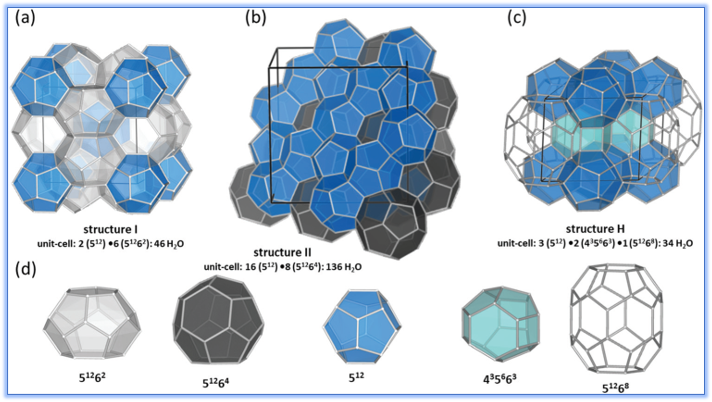
\includegraphics[width=.9\linewidth]{figures/hydrstruct.png}
    \caption{Кристаллическая структура трех наиболее распространенных типов гидратов, а также 5 различных полостей, образующих их. Источник[Gas hydrates in sustainable chemistry / A. Hassanpouryouzband [et al.] // Chem. Soc. Rev. – 2020. – Vol. 49. – P. 5225]}
    \label{fig1.2.1}
\end{figure}

\par Газовые гидраты состоят из воды на 85\% и по этой причине их часто сравнивают с обычным льдом. Однако в отличие от кристаллической решетки льда, характерная для гидратов структура не может существовать в отсутствие молекул-гостей. Кроме того, гидраты отличаются большей механической прочностью по сравнению со льдом[], обладают меньшей теплопроводностью[] и большей теплоемкостью по сравнению с гексагональным льдом.

\par Важно отметить, что газовые гидраты являются нестехиометричными соединениями и идеальных кристаллов газовых гидратов не существует, поскольку молекулы воды всегда присутствуют в большем  количестве чем молекулы газов. Поэтому еще одной характеристикой гидратов является число заполнения полостей. Идеальное стехиометрическое отношение для структуры \textit{sI} составляет $1:5^{3/4}$, \textit{sII} и \textit{sH} -- $1:5^{2/3}$ [].

\pagebreak
\section{Образование гидратов}
\par Процесс формирования гидратов принято разделять на стадию нуклеации и стадию устойчивого роста кристаллической фазы. Образование газовых гидратов из растворенных в воде газов возможно только в условиях низких температур и высоких давлений. В случае неполярных молекул-гостей, например, метана причина этого заключается в том, что \ce{CH4} является гидрофобной молекулой и имеет низкую величину растворимости в воде порядка $10^{-3}-10^{-5}$ мольных долей при обычных условиях. Однако при понижении температуры до отрицательных величин и увеличения давления до десятков МПа, растворимость  \ce{CH4} увеличивается на два порядка.

\par При исследовании клатратных гидратов под нуклеацией обычно подразумевают явление гомогенной нуклеации, которое представляет собой возникновение в исходной фазе чистого, то есть без наличия примесных молекул или атомов, вещества зародыша новой кристаллической или аморфной фазы, который может состоять из десятков или тысяч частиц. В объеме переохлажденной жидкости вследствие флуктуаций периодически образуются и распадаются кластеры (зародыши) из молекул воды, выстраивающихся вокруг растворенного метана.

\par Зародышеообразование является стохастическим явлением: с некоторой вероятностью зародыш может достичь некоторого критического размера $r$, после чего происходит устойчивый рост новой твердой фазы. Существование критического размера можно объяснить если обратить внимание на величину избытка свободной энергии Гиббса $\Delta G$, который равен сумме поверхностной и объемной частей свободных энергий зародыша:

\begin{equation}
\Delta G = \Delta G_{surf} + \Delta G_{vol} = 4\pi r^2 \sigma + \frac{3}{4}\pi r^3 \Delta g_{vol} \, .
\label{eq1.3.1}
\end{equation}

Здесь $\sigma$ -- поверхностное натяжение на границе раздела зародыша новой фазы и раствора, $\Delta g_{vol}$ изменение свободной энергии в пересчете на единицу объема. Как видно из рисунка \ref{fig1.3.1} $\Delta G$ имеет максимум, соответствующий критическому значению радиуса, который равен

\begin{equation}
    r_{crit} = -2\sigma/\Delta g_{vol} \,.
    \label{eq1.3.2}
\end{equation}
Соотношение \ref{eq1.3.2} можно получить, взяв производную \ref{eq1.3.1} по радиусу зародыша и приравняв её нулю. Соответствующий максимум избытка свободной энергии имеет вид
\begin{equation}
    \Delta G_{crit} = 4\pi\sigma r_{crit}^2 / 3 \,.
    \label{eq1.3.3}
\end{equation}

\begin{figure}[H] 
    \centering
    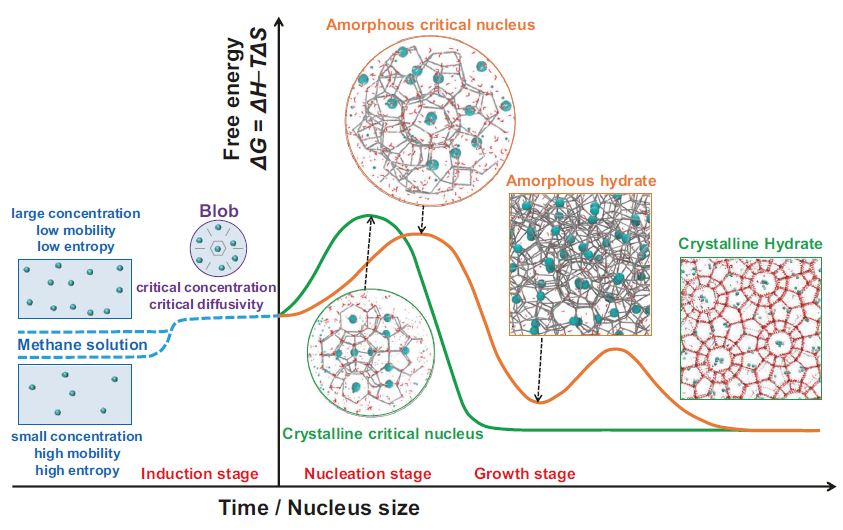
\includegraphics[width=.9\linewidth]{figures/hydrnucl.png}
    \caption{Диаграмма, иллюстрирующая рост гидрата метана. Источник[]}
    \label{fig1.3.1}
\end{figure}

Частота с которой возникают зародыши критического размера в значительной степени зависит от высоты энергетического барьера. При уменьшении величины $r_{crit}$ величина $\Delta G$ так же падает. Критический радиус зародыша может уменьшаться в зависимости от величины пересыщения и переохлаждения $\Delta T$ раствора по зависимости $r_{crit} \propto 1/\Delta T$[]. Соответственно увеличивается и вероятность зародышеообразования. 

В настоящее время считается, что образованию зародыша критического размера предшествует возникновение так называемого \textit{сгустка} (с англ. \textit{blob}) -- аморфного кластера, состоящего из нескольких молекул газа, разделенных между собой молекулами воды, возникающего вследствие локальных флуктуаций концентрации гостей. Концентрация молекул газов в сгустке выше чем, во всем остальном растворе, с которым он находится в динамическом равновесии. В пределах сгустка периодически возникают и исчезают гидратные полости и их фрагменты, адсорбируя окружающий газ и вновь концентрируя его. Впоследствии может возникнуть кластер критического размера. Критический зародыш может быть как аморфным, так и кристаллическим, в зависимости от того, какие типы полостей образуются первоначально. Соответственно возникает либо аморфная фаза гидрата, которая потом преобразуется в кристаллическую сама по себе со временем или путем отжига, либо же кристалл образуется напрямую.